\subsection{Test framework}
As discussed in previous sections, the model is to be used as a state observer for the Hi-Fi simulation. Since the linearised model did not have observability it was necessary to perform a Kalman decomposition. The model was reduced from 10 to 8 states in \cref{sec:kalman}. The reduced model will be referred to as the control model. \\

\noindent The control model must initially be tested to accurately estimate the observable states of the  10-state linearised model from \cref{sec:linearised-model}. In the test framework, the two models run in parallel, with the control signals $u$ equally applied to both systems. The control signals are computed by the controller K, based on the states of the control model. This framework is seen in \cref{fig:sim_modelSS_obs}. \\

\noindent As described in \cref{sec:observer-gain} a Luenberger observer gain $L$ was calculated. Any error between the actual output and estimated output will be multiplied by $L$ and added to the observer estimated states $\dot{\hat{x}}$. If $A-LC$ is stable, this topology will ensure $\hat{y}$ converges to $y$. If the states are observable (which the Kalman Decomposition ensures) and there is no present disturbance then $\hat{x}$ will converge to $x$. If a disturbance is present, the proportional observer gain will not be sufficient to estimate the states, and integral action should be included. For the purpose of these tests however, the error introduced by the disturbance is not handled by integral observer action. \\

\noindent For this test, the ambient temperature is set to 20$^{\circ}$C, which is its operating point value, such that no disturbance is present. This is clear by recalling that $\tilde{d} = d-d_o$. All states are initialized to the arbitrary value 1 to verify that all states are driven to zero and that the observed state vector $\hat{x}$ converges to $x$. It is recalled that in this coordinate system $x=0$ means $x-x_o = 0 \rightarrow x=x_o$. The control signal u is defined as $u=K\hat{x}$.


\begin{figure}[h!]
	\centering
	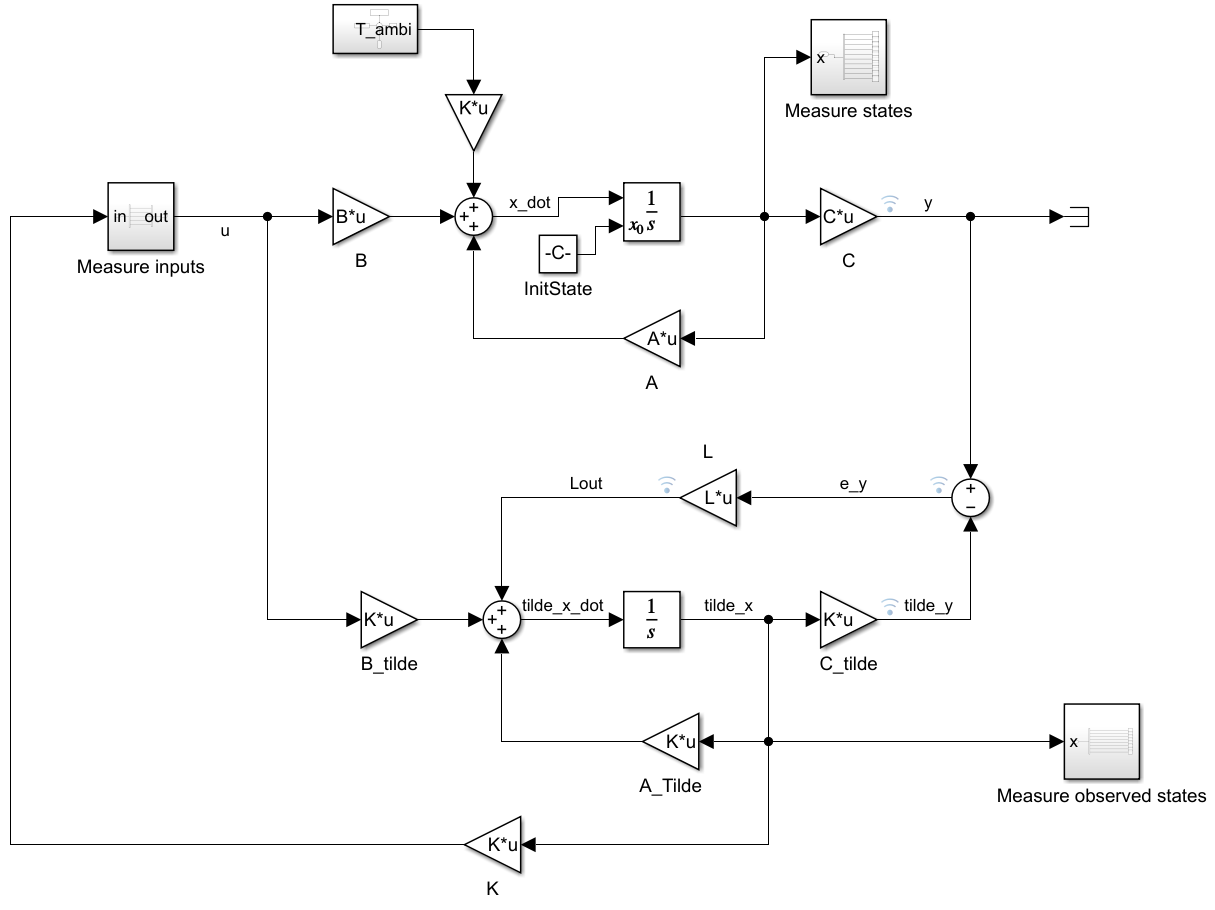
\includegraphics[width=0.9\textwidth]{Graphics/fig_modelSS_obs.png}
	\caption{The Matlab Simulink simulation model of the linearised system with feedback from Kalman Decomposition observer}
	\label{fig:sim_modelSS_obs}
\end{figure}

\newpage
\subsection{Test results}
The simulation was run for 10 hours to allow all states to settle. Four plots are made. In \cref{fig:sim_stateInput10h} a plot containing the state deviations and input deviations is seen of the linearised 'plant' model. All states converge to zero, indicating that the linearised model is stable. All states except the box temperature converge to steady state with about half an hour. The box temperature settles after about 8-9 hours. It is also noted that the inputs stay inside a reasonable interval, far from saturation of the actuators. The actuator ranges are 0 - 100, and with the $ u_0 $ given in \cref{tab:Inputs_ref} and the input deviations being less than $ |8| $, the inputs are well inside the actual range of the actuators.
\begin{table}[h]
	\centering
	\caption{Input operating points, $ u_0 $}
	\label{tab:Inputs_ref}
	\begin{tabular}{@{}lll@{}}
		\toprule
		\textbf{Inputs} & \textbf{\begin{tabular}[c]{@{}l@{}}Numeric \\ values\end{tabular}} & \textbf{Unit} \\ \midrule
		$\Theta_1$      & 19.4                                                               & \%            \\
		$U_{fan2}$      & 63.8                                                               & \%            \\ \bottomrule

	\end{tabular}
\end{table}

\begin{figure}[h!]
	\centering
	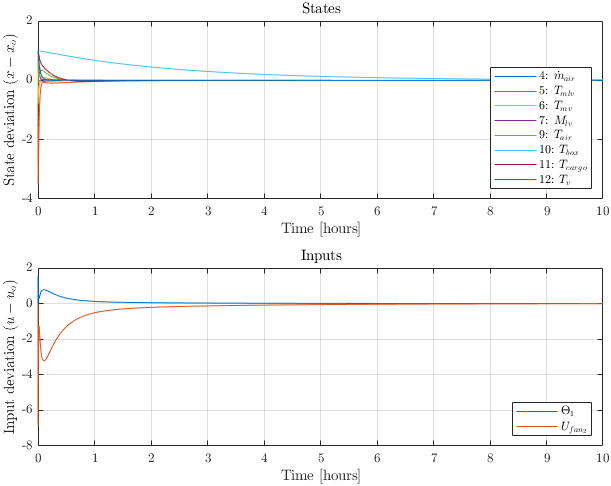
\includegraphics[width=1\textwidth]{Graphics/fig_stateInput10h.png}
	\caption{State and input deviations plotted for 10 hours. All states settle within an hour except the box temperature which settles in about 7-8 hours. The state deviations of the plant model is seen in subplot 1, and the input deviations to the plant model is seen in subplot 2.}
	\label{fig:sim_stateInput10h}
\end{figure}

\newpage
\noindent In \cref{fig:sim_stateInput1h} the same plot as previously is seen but zoomed in at 1 hour such that the behavior of the states is more easily observed. All of the states appear to be well damped.

\begin{figure}[h!]
	\centering
	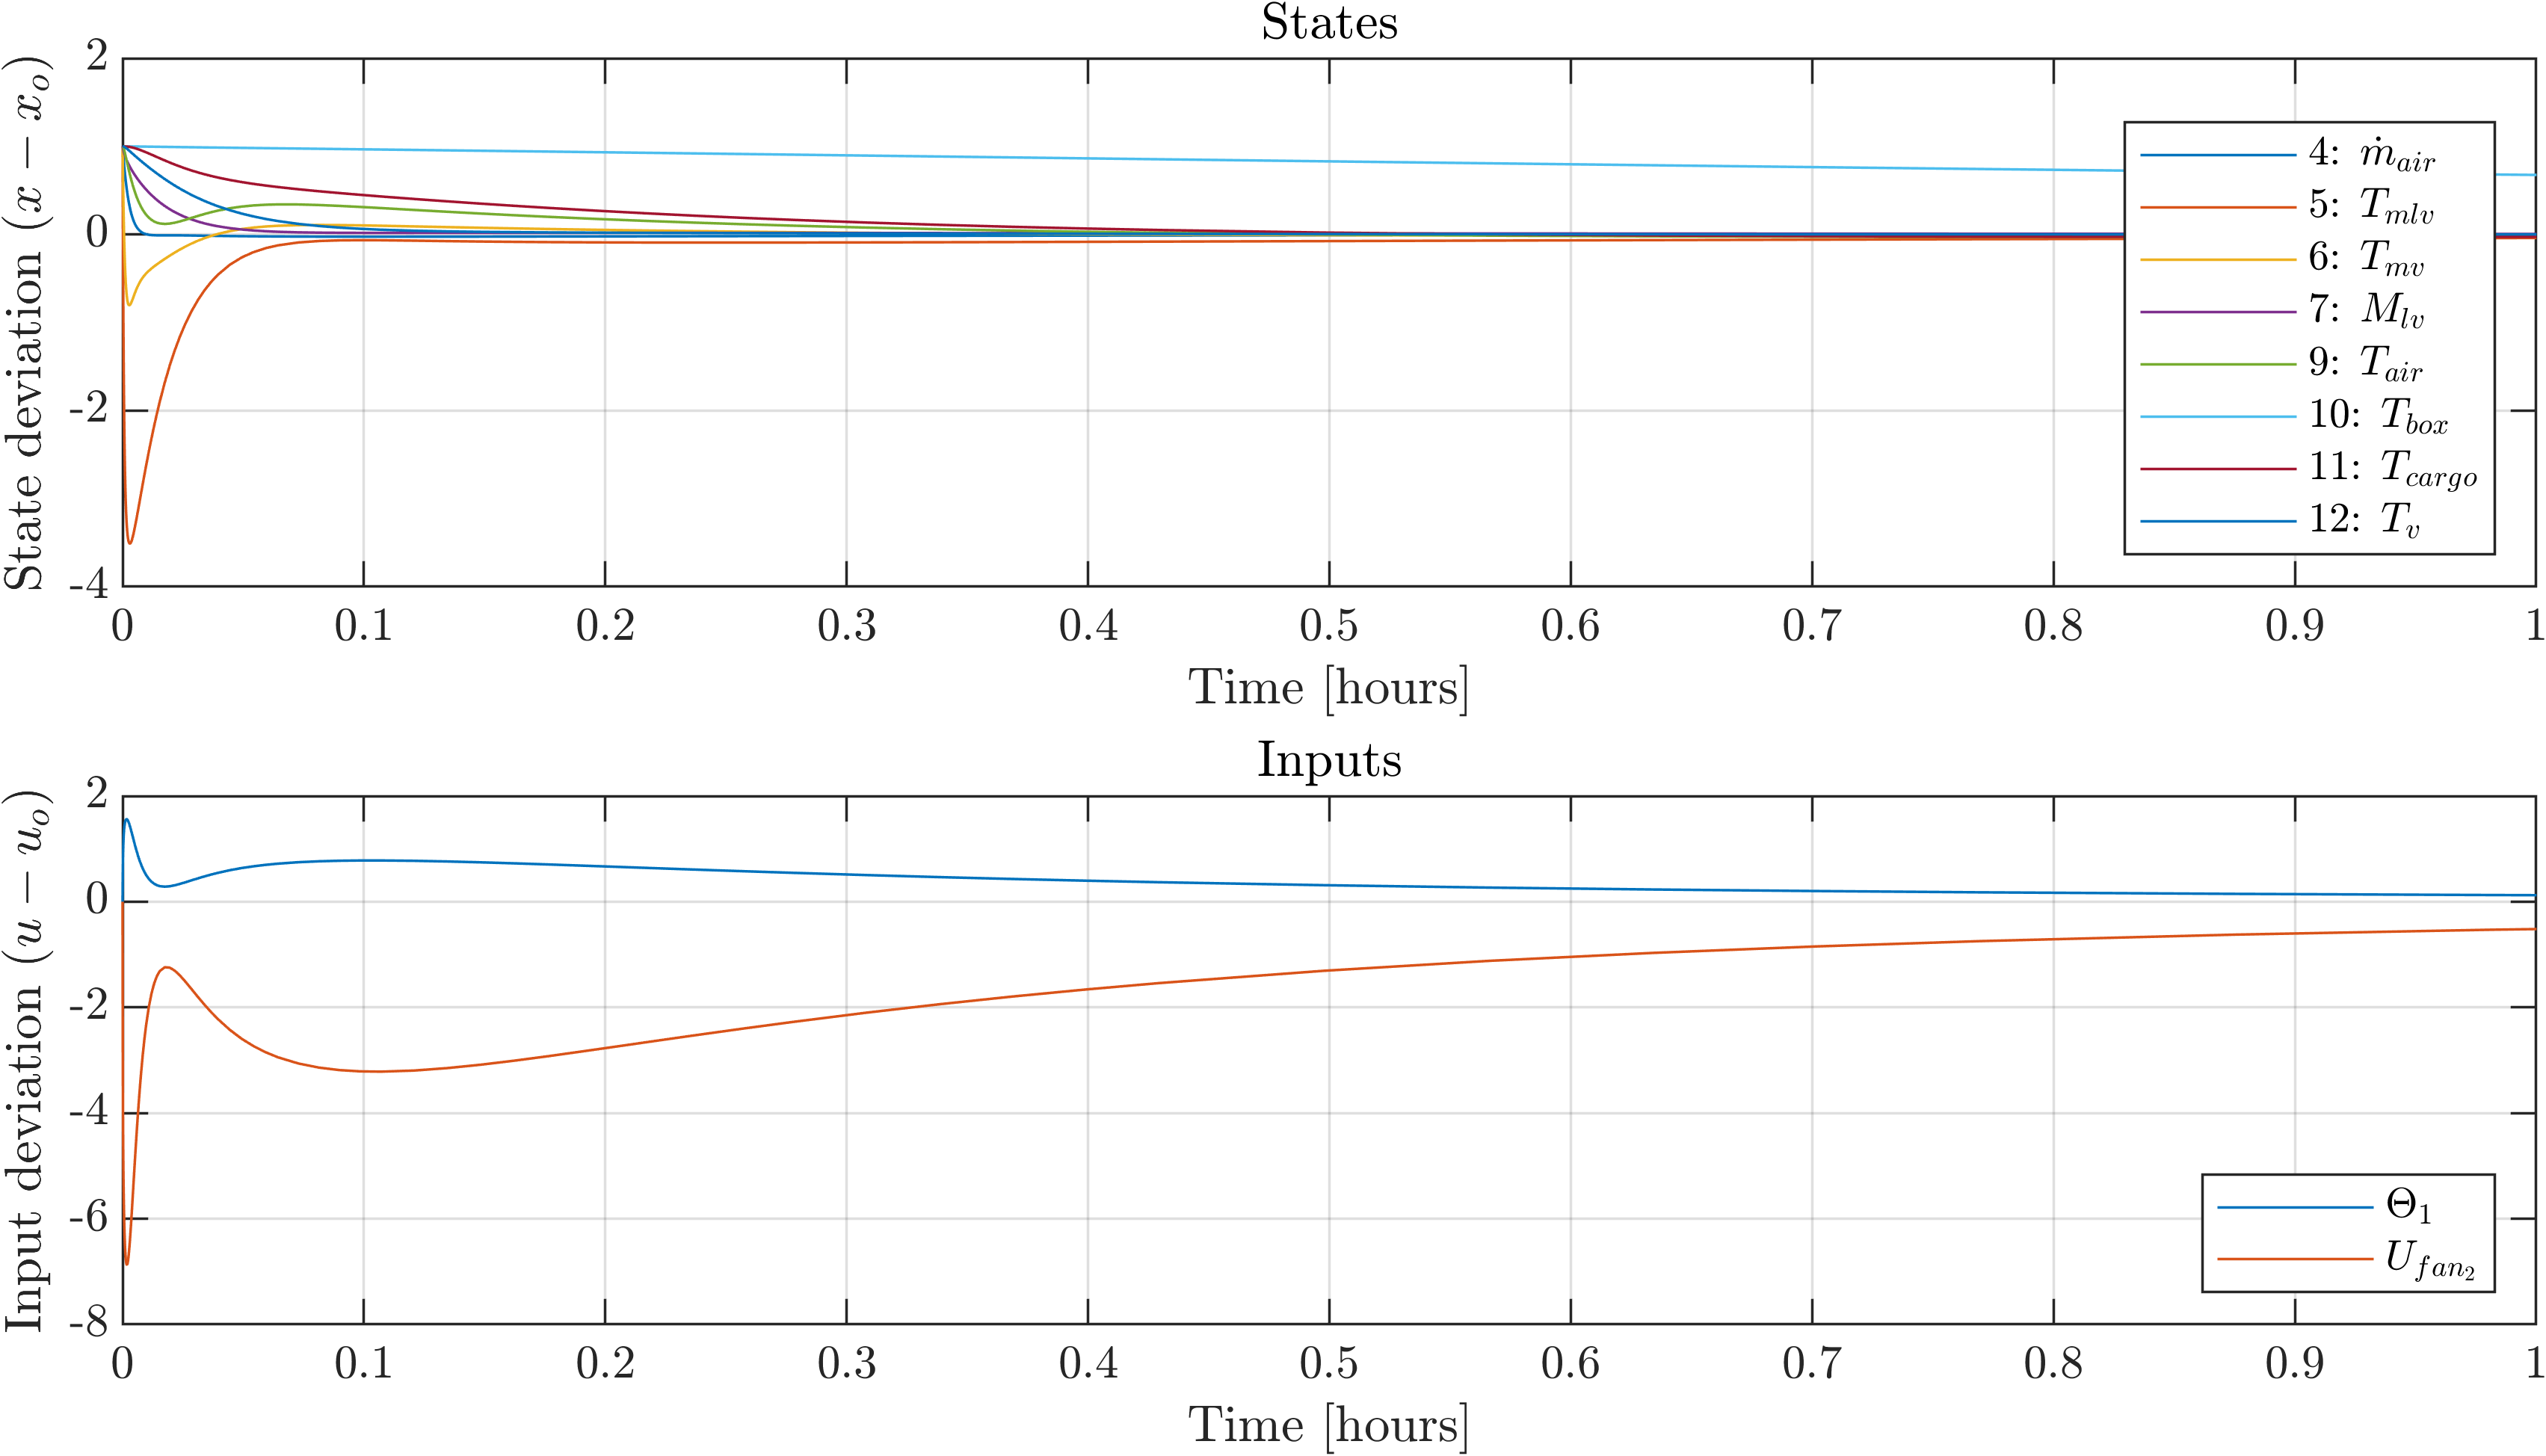
\includegraphics[width=1\textwidth]{Graphics/fig_stateInput1h.png}
	\caption{Zoomed version of \cref{fig:sim_stateInput10h}. States and inputs plotted for 1 hour. The states of the plant model is seen in subplot 1, and the inputs to the plant model is seen in subplot 2.}
	\label{fig:sim_stateInput1h}
\end{figure}

\newpage
\noindent In \cref{fig:sim_stateObsState1h} the state deviations are plotted in subplot 1 as is the observed state deviations in subplot 2. Additionally in subplot 3, the states and observed states are subtracted to highlight the difference between the two. It is seen that the observed states settle onto the actual states in around 0.2 hours, expect from the box temperature, that does not settle within one hour.

\begin{figure}[h!]
	\centering
	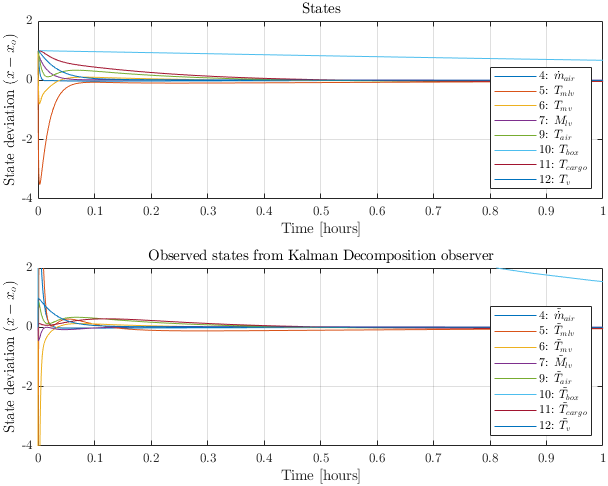
\includegraphics[width=1\textwidth]{Graphics/fig_stateObsState1h.png}
	\caption{States and Kalman Decomposition observed states plotted for 1 hour. The estimated box temperature obviously deviates from the actual state but begins to settle towards the correct state value. The other observed states settle within 0.2 hours.}
	\label{fig:sim_stateObsState1h}
\end{figure}

\newpage
\noindent In \cref{fig:sim_stateObsState002h} further zoom is made on the time axis to observe the fast transients in the first seconds of the simulation where the observer converges from the big starting error. It can be seen that the observed states initially in the first seconds deviate greatly before settling close to the actual states. The maximum absolute deviations are respectively the metal temperature $ T_{mv} - \tilde{T_{mv}} \approx 16$ and $ T_{cargo} - \tilde{T_{cargo}} \approx 9 $

\begin{figure}[h!]
	\centering
	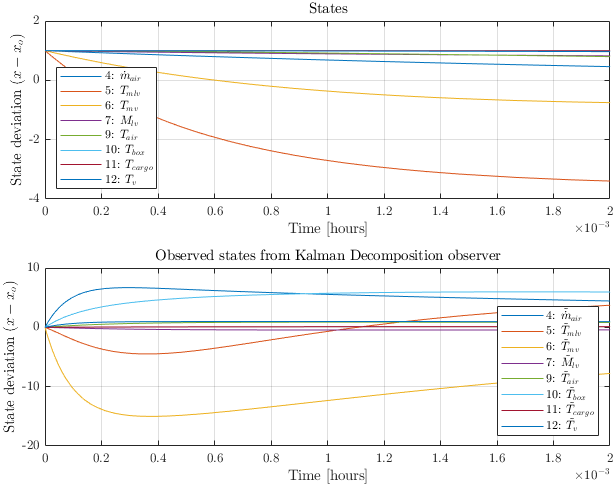
\includegraphics[width=1\textwidth]{Graphics/fig_stateObsState002h.png}
	\caption{Zoomed version of \cref{fig:sim_stateObsState1h}. States and Kalman Decomposition observed states plotted for 0.02 hours. Large deviations observed in the first seconds before observed states converge.}
	\label{fig:sim_stateObsState002h}
\end{figure}

Conclusively the test is a success. The linear state space model with observer  and controller simulates and is stable. The Kalman decomposition reduced model used as an observer also performs well and is able to settles onto the states nicely and in timely fashion. The next section will cover the observer and controller connected to the HiFi simulation model.
